\documentclass[twocolumn, a4paper]{article}
\usepackage[a4paper, left = 1.75cm, right = 1.75cm, top = 1.75cm, bottom = 1.75cm]{geometry}
\usepackage[style = numeric, sorting = none]{biblatex}
\usepackage{pgfplots}
\usepackage[T1]{fontenc}
\usepackage{graphicx}
\usepackage[UKenglish]{babel}
\usepackage[UKenglish]{isodate}

\graphicspath{{./images/}}
\addbibresource{refs.bib}

\cleanlookdateon

\renewcommand*{\bibfont}{\footnotesize}

\author{
  George Herbert\\
  \texttt{cj19328@bristol.ac.uk}
}

\title{\vspace{-2em}Parallelising d2q9-bgk.c with MPI}

\begin{document}

\maketitle

\begin{abstract}
  \texttt{d2q9-bgk.c} implements the Lattice Boltzmann method (LBM) to simulate a fluid density on a lattice.
  This report analyses the techniques I utilised to parallelise \texttt{d2q9-bgk.c} with MPI, and port \texttt{d2q9-bgk.c} to a GPU with OpenCL.
\end{abstract}

\section{Single Program, Multiple Data}

Single program, multiple data (SPMD) is a form of parallelism in which independent processes run the same program.
Message Passing Interface (MPI) is a specification for a library interface for passing messages between processes.

\subsection{Hypothesis}

I previously achieved a substantial performance improvement parallelising sections of my code with OpenMP.
The most notable improvement came from executing 28 iterations of the inner loop in the \texttt{timestep} function in parallel.
To accomplish this, OpenMP launched 28 threads, each of which ran on one of the 28 cores of a BC4 compute node.
Naturally, I conjectured that an even greater performance improvement could be achieved by utilising more than 28 cores.
However, OpenMP was designed for shared-memory parallelism, and so was restricted to a single node---a considerable restriction considering BC4 contained hundreds of nodes.
Therefore, I hypothesised that I could use the Intel MPI Library to execute \texttt{d2q9-bgk.c} on multiple processes across multiple nodes in parallel, which would provide an even more significant performance improvement.

\subsection{Implementation}

I selected to use the final implementation of my program before single instruction, multiple data (SIMD) vectorization as my starting point.

\begin{figure}[htbp]
  \centering
  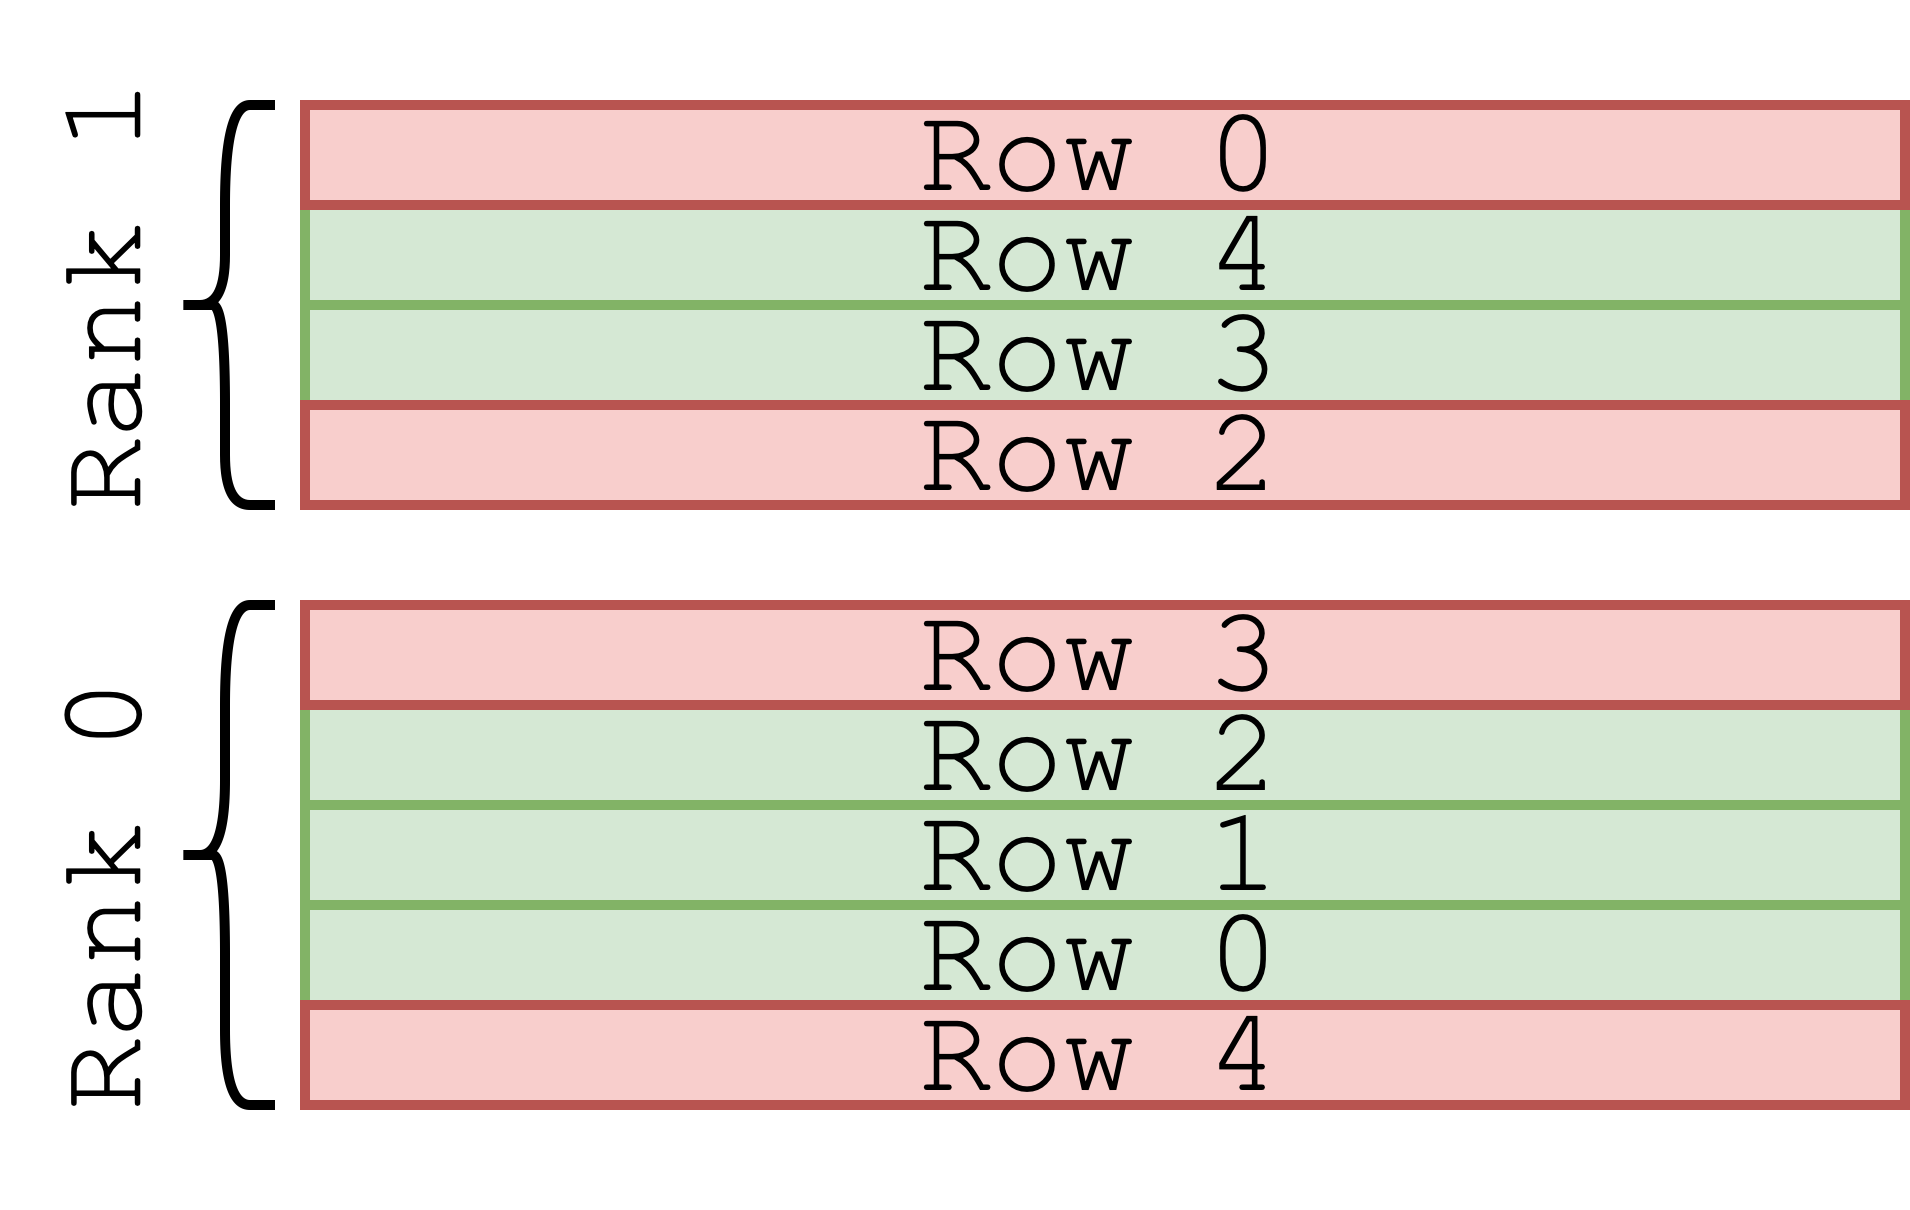
\includegraphics[width=.75\linewidth]{rows.png}
  \caption{Row allocation example with five rows and two processes}\label{fig:rows}
\end{figure}

Since the \texttt{cells} grid was stored in row-major order, I chose to split the grid horizontally between processes to take advantage of memory locality.
I created a procedure \texttt{allocate\_rows} to balance the load; the procedure assigned each process at least $\lfloor\frac{y}{n}\rfloor$ consecutive rows, with the first $y - \lfloor\frac{y}{n}\rfloor n$ processes each assigned an additional row, where $y$ was the number of rows and $n$ the number of processes.
This was the most equal way to allocate cells to processes without splitting on a sub-row level, which I decided against to avoid increasing the complexity of my program and incurring an additional computational overhead.
Additionally, since updating the value of a given cell required the values of all adjacent cells, each process contained two additional rows reserved for cells in the top and bottom rows of the preceding and succeeding ranks, respectively.
Figure \ref{fig:rows} displays an example allocation for a grid with five rows, split between two processes; the rows allocated to a specific process are highlighted in green, with additional rows required to correctly updated the edge rows highlighted in red.

Since processes have their own memory space, I had to explicitly send the contents of cells between processes.
To do so, I created a \texttt{halo\_exchange} procedure.
More specifically, at the end of each timestep, the bottom-most row allocated to each process was copied into the \texttt{send\_row\_buffer} array.
I used the \texttt{MPI\_Sendrecv} procedure to send this buffer to the \texttt{receive\_row\_buffer} of the preceding rank.
The same process was then repeated for the top-most row, which was sent to the succeeding rank.

After all iterations have been complete, each process (with the exception of rank zero) sends the final state of its \texttt{cells} grid section to rank zero with the \texttt{MPI\_Send} procedure.
Rank zero receives each section using the \texttt{MPI\_Recv} procedure.

To compute the average velocities at each timestep.

\subsection{Results}

\begin{table}[htbp]
  \begin{center}
  \caption{Execution times with the 52 process MPI implementation and speedup over both the prior and 28 thread OpenMP implementation}\label{tab:mpi}
  \begin{tabular}[t]{l | l  l  l} 
      \hline\hline
      &&\multicolumn{2}{c}{Speedup}\\
      \cline{3-4}
      Grid Size&Time (s)&Prior&OpenMP\\
      \hline
      $128 \times 128$&\texttt{}&\texttt{}&\texttt{}\\
      $128 \times 256$&\texttt{}&\texttt{}&\texttt{}\\
      $256 \times 256$&\texttt{}&\texttt{}&\texttt{}\\
      $1024 \times 1024$&\texttt{}&\texttt{}&\texttt{}\\
      \hline
    \end{tabular}
  \end{center}
\end{table}

Each time was an average of five runs on a BlueCrystal Phase 4 (BC4) compute node---a Lenovo nx360 M5, which contained two 14-core 2.4 GHz Intel E5-2680 v4 (Broadwell) CPUs and 128 GiB of RAM \cite{bcp4}.

\section{Experiments}

\subsection{Vectorization}

I hypothesised that SIMD vectorization of the inner loop would drastically improve the performance of my MPI implementation, as it did with my serial optimised implementation previously.
Therefore, I made the same changes as I did with my serial optimised implementation, including converting the cells' data from an array of structures (AoS) to a structure of arrays (SoA) format.
However, the SoA format meant that the \texttt{halo\_exchange} procedure had to be altered since the \texttt{MPI\_Sendrecv} procedure required the address of a single buffer as input.

I experimented with two separate approaches to send a row in the \texttt{halo\_exchange} procedure.
The first approach involved nine separate calls to the \texttt{MPI\_Sendrecv procedure}, one for each of the nine arrays in the SoA.
The second approach involved copying the cells' values in each of the nine arrays into a large buffer, followed by a single call to the \texttt{MPI\_Sendrecv} procedure.

Table \ref{tab:vectorization_1} and Table \ref{tab:vectorization_2} display the results for the first and second approach, respectively.
The second approach was significantly faster, since the overhead introduced by nine separate calls to the \texttt{MPI\_Sendrecv} procedure was larger than the overhead introduced by copying the values within the nine arrays into a single buffer.

\begin{table}[htbp]
  \begin{center}
  \caption{Execution times with the first vectorization approach and speedup over the prior implementation}\label{tab:vectorization_1}
  \begin{tabular}[t]{l | l l} 
      \hline\hline
      Grid Size&Time (s)&Speedup\\
      \hline
      $128 \times 128$&\texttt{}&\texttt{}\\
      $128 \times 256$&\texttt{}&\texttt{}\\
      $256 \times 256$&\texttt{}&\texttt{}\\
      $1024 \times 1024$&\texttt{}&\texttt{}\\
      \hline
    \end{tabular}
  \end{center}
\end{table}

\begin{table}[htbp]
  \begin{center}
  \caption{Execution times with the second vectorization approach and speedup over the prior implementation}\label{tab:vectorization_2}
  \begin{tabular}[t]{l | l l} 
      \hline\hline
      Grid Size&Time (s)&Speedup\\
      \hline
      $128 \times 128$&\texttt{}&\texttt{}\\
      $128 \times 256$&\texttt{}&\texttt{}\\
      $256 \times 256$&\texttt{}&\texttt{}\\
      $1024 \times 1024$&\texttt{}&\texttt{}\\
      \hline
    \end{tabular}
  \end{center}
\end{table}

\subsection{Hybrid MPI and OpenMP}

I also experimented with a hybrid MPI and OpenMP implementation.
In this implementation, each of the four compute nodes contained a single process.

\begin{table}[htbp]
  \begin{center}
  \caption{Execution times with the hybrid implementation and speedup over the prior implementation}\label{tab:hybrid}
  \begin{tabular}[t]{l | l l} 
      \hline\hline
      Grid Size&Time (s)&Speedup\\
      \hline
      $128 \times 128$&\texttt{}&\texttt{}\\
      $128 \times 256$&\texttt{}&\texttt{}\\
      $256 \times 256$&\texttt{}&\texttt{}\\
      $1024 \times 1024$&\texttt{}&\texttt{}\\
      \hline
    \end{tabular}
  \end{center}
\end{table}

\subsection{OpenMP vs MPI}

\begin{figure}[htpb]
  \centering
  \resizebox{\columnwidth}{!}{
    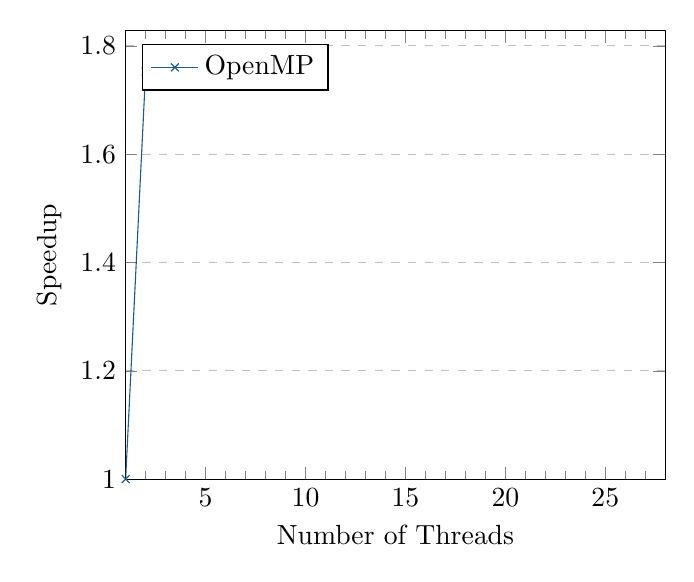
\begin{tikzpicture}
      \begin{axis}[
        xlabel={Number of Threads},
        ylabel={Speedup},
        xmin = 1, xmax = 28,
        ymin = 1,
        % xtick={0, 5, 10, 15, 20, 25},
        % ytick={0,20,40,60,80,100,120},
        legend pos=north west,
        ymajorgrids=true,
        grid style=dashed,
        minor xtick = {1, 2, 3, 4, 5, 6, 7, 8, 9, 10, 11, 12, 13, 14, 15, 16, 17, 18, 19, 20, 21, 22, 23, 24, 25, 26, 27, 28}
      ]
      \addlegendentry{OpenMP}
      \addplot[color = {rgb:red,31;green,119;blue,180}, mark = x]coordinates{
        (1, 1.0)
        (2, 1.7525169788462858)
      };
      \addlegendentry{MPI}
      \addplot[color = {rgb:red,255;green,127;blue,14}, mark = x]coordinates{
      };
      \end{axis}
    \end{tikzpicture}
  }
  \caption{Speedup curves for my OpenMP and MPI implementation on the $1024\times1024$ grid}\label{fig:scaling_openmp_mpi}
\end{figure}

\subsection{Scaling}

\begin{figure}[htpb]
  \centering
  \resizebox{\columnwidth}{!}{
    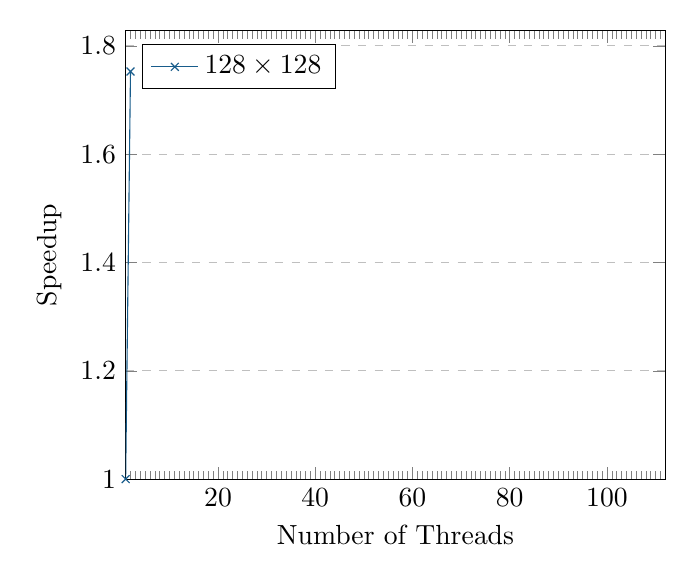
\begin{tikzpicture}
      \begin{axis}[
        xlabel={Number of Threads},
        ylabel={Speedup},
        xmin = 1, xmax = 112,
        ymin = 1,
        % xtick={0, 5, 10, 15, 20, 25},
        % ytick={0,20,40,60,80,100,120},
        legend pos=north west,
        ymajorgrids=true,
        grid style=dashed,
        minor xtick = {1, 2, 3, 4, 5, 6, 7, 8, 9, 10, 11, 12, 13, 14, 15, 16, 17, 18, 19, 20, 21, 22, 23, 24, 25, 26, 27, 28, 29, 30, 31, 32, 33, 34, 35, 36, 37, 38, 39, 40, 41, 42, 43, 44, 45, 46, 47, 48, 49, 50, 51, 52, 53, 54, 55, 56, 57, 58, 59, 60, 61, 62, 63, 64, 65, 66, 67, 68, 69, 70, 71, 72, 73, 74, 75, 76, 77, 78, 79, 80, 81, 82, 83, 84, 85, 86, 87, 88, 89, 90, 91, 92, 93, 94, 95, 96, 97, 98, 99, 100, 101, 102, 103, 104, 105, 106, 107, 108, 109, 110, 111, 112}
      ]
      \addlegendentry{$128\times128$}
      \addplot[color = {rgb:red,31;green,119;blue,180}, mark = x]coordinates{
        (1, 1.0)
        (2, 1.7525169788462858)
      };
      \addlegendentry{$128\times256$}
      \addplot[color = {rgb:red,255;green,127;blue,14}, mark = x]coordinates{
      };
      \addlegendentry{$256\times256$}
      \addplot[color = {rgb:red,44;green,160;blue,44}, mark = x]coordinates{
      };
      \addlegendentry{$1024\times1024$}
      \addplot[color = {rgb:red,214;green,39;blue,40}, mark = x]coordinates{
      };
      \end{axis}
    \end{tikzpicture}
  }
  \caption{Speedup curves for my MPI implementation}\label{fig:scaling}
\end{figure}

\section{Comparison to Serial}

\section{GPU Programming}

\subsection{Original Code}

\begin{table}[htbp]
  \begin{center}
  \caption{Execution times with the OpenCL implementation and speedup over the serial implementation}\label{tab:OpenCL_1}
  \begin{tabular}[t]{l | l l} 
      \hline\hline
      Grid Size&Time (s)&Speedup\\
      \hline
      $128 \times 128$&\texttt{}&\texttt{}\\
      $128 \times 256$&\texttt{}&\texttt{}\\
      $256 \times 256$&\texttt{}&\texttt{}\\
      $1024 \times 1024$&\texttt{}&\texttt{}\\
      \hline
    \end{tabular}
  \end{center}
\end{table}

\subsection{Optimisations}

\begin{table}[htbp]
  \begin{center}
  \caption{Execution times with the OpenCL implementation and speedup over the prior implementation}\label{tab:OpenCL_2}
  \begin{tabular}[t]{l | l l} 
      \hline\hline
      Grid Size&Time (s)&Speedup\\
      \hline
      $128 \times 128$&\texttt{}&\texttt{}\\
      $128 \times 256$&\texttt{}&\texttt{}\\
      $256 \times 256$&\texttt{}&\texttt{}\\
      $1024 \times 1024$&\texttt{}&\texttt{}\\
      \hline
    \end{tabular}
  \end{center}
\end{table}

\section{Conclusion}

\printbibliography

\end{document}